\documentclass[11pt,a4paper]{report}
\usepackage[latin1]{inputenc}
\usepackage[T1]{fontenc}  
\usepackage[french]{babel}
\usepackage{url}
\usepackage{graphicx}
\usepackage{fancyhdr}
\pagestyle{fancy}
\usepackage{listings}


\title{Rapport de projet : Architecture des ordinateurs}
\author{Benjamin Saint-Sever, Steven Ratton}
\date{\today}

\renewcommand{\headrulewidth}{1pt}
\fancyhead[R]{Rapport de Projet}

\renewcommand{\footrulewidth}{1pt}
\fancyfoot[L]{Rapport de projet}


\begin{document}

\maketitle

\tableofcontents





\chapter{Introduction}
Le but de ce projet est de montrer la possibilit� d'extension de l'architecture y86, en ajoutant des instructions et en manipulant les pr�dictions de branchement. Ce projet a pour vocation de nous enseigner la programmation de langage machine tout en tirant parti au mieux des capacit�s des ordinateurs. 

\chapter {Exercice 1}
\section{impl�mentation de leal}
\paragraph{Description\\}

Le but de ce premier exercice est de cr�er une nouvelle instruction "leal" pour "load effective address", cette derniere est existante sous l'architecture x86. Cette instruction charge l'adresse de la source dans dest ( leal (\%regS),\%regD). On souhaite que cette instruction permette un d�placement m�moire, leal depl(\%regS),regD. L'avantage de cette solution est que l'on peut effectuer cette op�ration avec une seule instruction. Son equivalent est : "rrmovl \%regS,\%regD ; iaddl depl,\%regD"
\newline

\paragraph{Assembleur\\}
Il est possible d'ajouter cette instruction sans consommer un nouvel opcode, il suffit de reprendre le formalisme de irmovl est de donner une valeur de ifun diff�rente afin de faire la distinction (ifun =1).

Premiere �tapes, on ins�re dans le code assembleur la d�claration de cette nouvelle instruction : 

\begin{enumerate}
\item isa.c
\begin{lstlisting}
   instr_t instruction_set[] = 
{
/*Ajout de leal avec iFun a 1*/
{"leal", HPACK(I_IRMOVL, 1), 6, M_ARG, 1, 0, R_ARG, 1, 1 },
\end{lstlisting}


\item yas-grammar.lex
\begin{lstlisting}
Instr         leal|rrmovl|rmmovl|mrmovl|irmovl|
\end{lstlisting}
\end{enumerate}

\newpage
\paragraph{Fichier test\_leal.ys : \\}

On d�place de 8 � partir de l'adresse du registre \%eax et on attribue l'adresse dans le registre \%ebx :

\begin{lstlisting}
 irmovl 3, %eax
        leal 8(%eax), %ebx
        halt
\end{lstlisting}

\paragraph{Code HCL : \\}
On ajoute le code d'instruction irmovl pour identifier leal:
\begin{lstlisting}
intsig LEAL     'I_IRMOVL'
\end{lstlisting}
\newpage

\section{Architecture s�quentielle}
\paragraph{Etape FETCH : \\}On ne modifie rien puisque l'on interpr�te le m�me fonctionnement que l'instruction irmovl.
\paragraph{Etape Decode :\\}le contenue du registre 'B' (Source) est attribu� � la source A.
\begin{lstlisting}
int srcA = [
        #icode vaut irmovl ou leal, pour obtenir leal -> ifun=1
        (icode == LEAL) && (ifun == 1):rB;
];
\end{lstlisting}
le contenue du registre 'A' est attribu� � la E destination afin d'�crire la nouvelle adresse de destination.
\begin{lstlisting}
int dstE = [
        (icode == IRMOVL) && (ifun == 0) : rB;
        (icode == LEAL) && (ifun == 1) : rA;
];
\end{lstlisting}

\paragraph{Etape Execute : \\} 
On place ValC dans l'aluA et ValA dans l'aluB, cela permettre d'effectuer le calcul de d�placement :
\begin{lstlisting}
int aluA = [
        (icode == IRMOVL) && (ifun == 0) : valC;
        (icode == LEAL) && (ifun == 1): valC;
];
int aluB = [
        (icode == IRMOVL) && (ifun == 0) : 0;
        (icode == LEAL) && (ifun == 1): valA;
];

\end{lstlisting}

\begin{figure}[h!]
  \centering 
  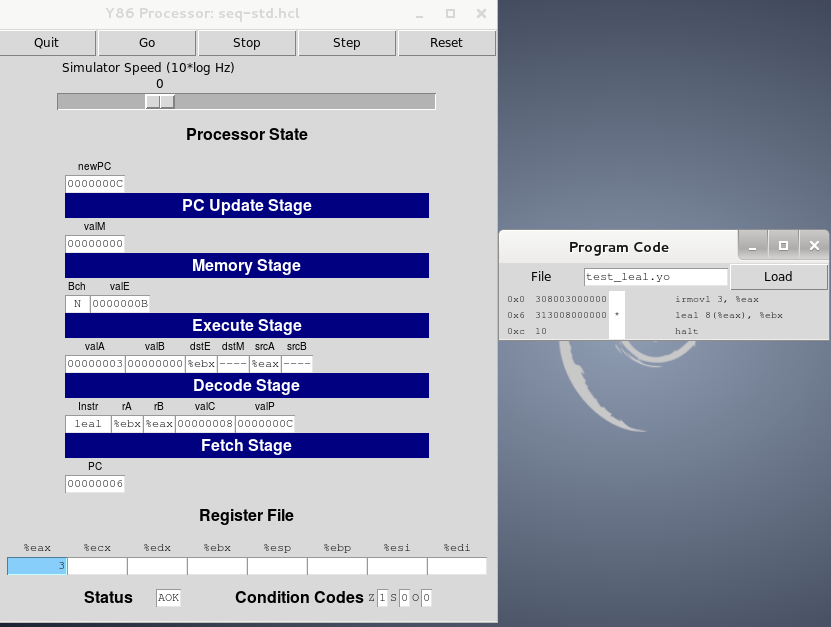
\includegraphics[height=9.5cm]{leal.png}
  \caption{Fetch}

\end{figure}

\begin{figure}[h!]
  \centering 
  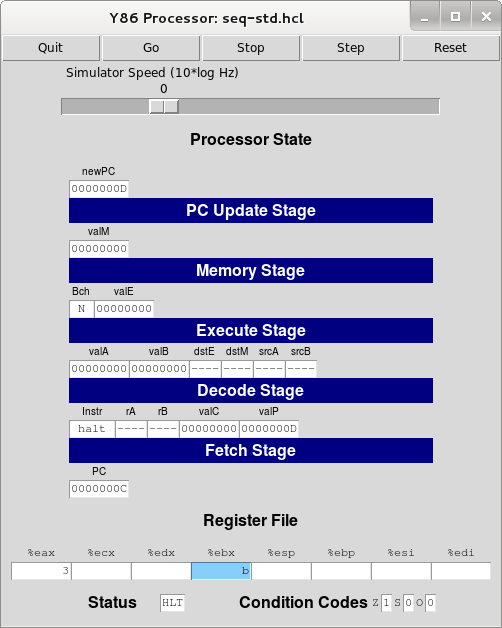
\includegraphics[height=9cm]{valeurleal.png}
  \caption{Decode}

\end{figure}
\clearpage
\newpage
\section{Architecture pipe\-lines}




\end{document}